\section{Products, inverse bounds, and the quantitative tradeoff}
\label{sec:consequences}

\subsection{A mixed-radix product preserves distance}

\begin{proposition}[Robust cyclic digit product]\label{prop:product}
Let \(v\ge1\) and \(N_i,s_i\ge2\) be integers.
For \(1\le i\le v\), let \(c_i:\Z/N_i\Z\to[s_i]\) be colorings
such that every nonzero-step \(k\)-term cyclic progression has
distance at least \(t_i\) from every constant word.
There is a coloring of \(\Z/Q\Z\), \(Q=\prod_{i=1}^vN_i\),
using \(\prod_i s_i\) colors, with distance at least
\(\min_i t_i\) on every nonzero-step \(k\)-term cyclic progression.
No coprimality hypothesis on the \(N_i\) is needed.
\end{proposition}

\begin{proof}
Put \(B_1=1\), \(B_i=\prod_{j<i}N_j\), and \(B_{v+1}=Q\).
The \(i\)-th digit of a residue \(n\), represented in \([0,Q)\), is
\[
 d_i(n)=\fl{n/B_i}\pmod{N_i}.
\]
Give \(n\) the tuple \((c_i(d_i(n)))_{i=1}^v\).
For a nonzero common difference represented by \(0<d<Q\), choose
the largest \(i\) with \(B_i\mid d\). Then \(N_i\nmid d/B_i\).
For unreduced integer values \(a+jd\),
\[
 \fl{(a+jd)/B_i}=\fl{a/B_i}+j(d/B_i).
\]
Reducing \(a+jd\) modulo \(Q\) subtracts a multiple of \(Q/B_i\)
from this quotient; that number is divisible by \(N_i\).
Thus the \(i\)-th digits on the cyclic progression form a
nonzero-step cyclic progression modulo \(N_i\).

For any fixed target color tuple, at least \(t_i\) positions differ
from its \(i\)-th component, and therefore differ from the tuple.
This proves the claim. It does not require other digit colors to
vary or every possible tuple color to occur.
\end{proof}

\begin{proposition}[Periodic extension to an interval]\label{prop:periodic}
A cyclic coloring of \(\Z/Q\Z\) with distance at least \(t\) on every
nonzero-step \(k\)-term progression extends to an interval of length
\((k-1)Q\) with the same property.
\end{proposition}

\begin{proof}
Repeat the coloring periodically on
\(\{0,\ldots,(k-1)Q-1\}\).
Any \(k\)-term progression of positive step \(d\) in this interval
has \((k-1)d<(k-1)Q\), so \(0<d<Q\).
Its reduction modulo \(Q\) therefore has nonzero step and the same
color word. Translate the interval by one if desired.
\end{proof}

The nonrobust version is the periodic transfer in
\cite[Lemma 2]{camposFoxSchildkraut2026}. The proof shows directly why
the same exact factor preserves the distance property.

\subsection{Exact optimization of the number of colors}

\begin{proposition}[Binary--ternary palette optimization]
\label{prop:palette}
For every integer \(r\ge2\),
\begin{equation}\label{eq:palette-max}
 \max_{\substack{a,b\in\Z_{\ge0}\\2^a3^b\le r}}
 \left(\frac a{24}+\frac b{18}\right)
 =\Lambda(r)
\end{equation}
with \(\Lambda(r)\) as in \eqref{eq:palette-coefficient}.
An optimizer uses \(a=m-e(r)\), \(b=e(r)\), hence exactly \(m\)
digit factors.
\end{proposition}

\begin{proof}
Two ternary digits use nine colors and contribute \(2/18=1/9\).
Three binary digits use only eight colors and contribute \(3/24=1/8\),
which is larger. Thus no optimum has \(b\ge2\).
If \(b=0\), the best choice is \(a=m=\fl{\log_2r}\).
If \(b=1\), feasibility of \(a=m-1\) is exactly
\(r\ge3\cdot2^{m-1}\). In this case it contributes
\[
 (m-1)/24+1/18=m/24+1/72.
\]
Otherwise \(a\le m-2\), and the ternary option is worse than \(m/24\).
The case \(m=1\) is covered by the same two alternatives \(r=2,3\).
\end{proof}

\begin{proof}[Proofs of \cref{thm:main-two,thm:main-many}]
For \(r=2\), use \cref{thm:cyclic} with \(s=2\), and
\cref{prop:periodic}. Take \(b=B/2\).

For arbitrary \(r\), use \(m-e(r)\) copies of the binary cyclic
coloring and \(e(r)\) copies of the ternary one.
Their total number of colors is at most \(r\), and the same integer
distance \(t=\fl{BE_k/2}\) works for every factor.
By \cref{prop:product} their product is cyclically robust.
The sum of their logarithmic sizes is at least
\[
 \Lambda(r)k(L-5\log L)-Cmk.
\]
Apply \cref{prop:periodic}. The constants and the threshold were
chosen for two palettes before \(r\) was introduced, proving the
uniformity in the theorem.
\end{proof}

This is an optimization within the stated binary and ternary
primitives. It does not claim optimality among every possible
coloring construction.

\subsection{Recoloring and deletion interpretations}

\begin{corollary}\label{cor:edits}
For the colorings of \cref{thm:main-many}, let
\(t=\fl{b k^{2/3}(\log k)^{5/3}}\).
Recoloring at most \(t-1\) vertices anywhere in the interval cannot
create a monochromatic \(k\)-term progression.
Deleting at most \(t-1\) positions from the color word of any original
\(k\)-term progression cannot make all its remaining positions one
color.
\end{corollary}

\begin{proof}
Every target color initially has at least \(t\) disagreements on every
progression. One recoloring or one deleted position removes at most
one of those disagreements.
\end{proof}

The deletion statement concerns the word of an original progression.
It does not say that the undeleted points themselves form an arithmetic
progression of a new length.

\subsection{Inverting the lower-bound scale}

Inversion has a concrete Ramsey interpretation here: it turns a
lower bound for \(W_2(k)\) into a guaranteed coloring on a prescribed
interval length. It does not produce an asymptotic formula for
\(W_2(k)\) itself.

\begin{corollary}[Prescribed interval size]\label{cor:inverse}
There are constants \(C',b'>0\) such that for every sufficiently
large integer \(n\), writing \(X=\log n\), there is a two-coloring
of \([n]\) with no monochromatic progression of length
\begin{equation}\label{eq:inverse-explicit}
 k_n=
 \cl{\frac{24X}
 {\log X-6\log\log X-C'}} .
\end{equation}
In fact every progression of that length contains at least
\[
 \fl{b'(\log n)^{2/3}\log\log n}
\]
positions of each color.
\end{corollary}

\begin{proof}
Let \(C\) be the constant of \cref{thm:cyclic} for two colors and put
\[
 F(u)=\frac u{24}(\log u-5\log\log u)-Cu.
\]
This is increasing for all sufficiently large \(u\).
For \(\ell=\log X\), \(v=\log\ell\), and
\(u=24X/(\ell-6v-C')\), direct expansion gives
\[
 \log u-5\log\log u-24C
 =\ell-6v+\log24-24C+O(v/\ell).
\]
Choose \(C'>24C-\log24+1\).
The numerator in this last expression exceeds
\(\ell-6v-C'\) for large \(X\), so \(F(u)\ge X\).
Taking the ceiling preserves this inequality.
The cyclic coloring for \(k_n\) has \(N_2\ge e^{F(k_n)}\ge n\),
and can be restricted to \([n]\).

Finally
\(k_n\sim24X/\ell\) and \(\log k_n\sim\ell\).
The distance in \eqref{eq:cyclic-robust} is therefore asymptotic to
\((B/2)24^{2/3}X^{2/3}\ell\). Reducing the constant gives the
stated lower bound.
\end{proof}

For readers wanting more terms, the smooth bound admits an ordinary
logarithmic reversion with a controlled remainder.

\begin{proposition}[Two correction polynomials]\label{prop:reversion}
Let \(\beta\) be fixed, and let \(u(Y)\) be the large positive solution
of
\[
 Y=u(\log u-5\log\log u-\beta).
\]
Put \(T=\log Y\), \(V=\log T\), and \(d=6V+\beta\).
Then
\begin{equation}\label{eq:reversion}
 u(Y)=\frac YT\left[
 1+\frac dT+\frac{d^2-d-5V}{T^2}
 +O\!\left(\frac{V^3}{T^3}\right)\right].
\end{equation}
For inversion of \(F\), take \(Y=24X\), \(\beta=24C\).
\end{proposition}

\begin{proof}
Substitute \(u=(Y/T)(1+A/T+D_2/T^2)\). Taylor expansion, uniformly
for \(A=O(V)\), \(D_2=O(V^2)\), gives
\[
 \log u=T-V+A/T+(D_2-A^2/2)/T^2+O(V^3/T^3),
\]
and
\[
 \log\log u=V-V/T+(A-V^2/2)/T^2+O(V^3/T^3).
\]
Multiplying \(u\) by the required bracket and dividing by \(Y\)
gives coefficients \(A-d\) at \(T^{-1}\), and
\(D_2-Ad+A+5V\) at \(T^{-2}\).
Set \(A=d\) and \(D_2=d^2-d-5V\); the residual is
\(O(V^3/T^3)\).
The derivative of \(u(\log u-5\log\log u-\beta)\) is asymptotic to
\(T\) in this range. The mean value theorem changes the candidate
by \(O(YV^3/T^4)\), proving \eqref{eq:reversion}.
\end{proof}

The exact smooth inverse followed by a ceiling is justified by
monotonicity. Rounding a truncated asymptotic expansion without an
error enclosure would not be justified.

\subsection{A fixed-power robustness tradeoff}

\begin{theorem}\label{thm:tradeoff}
Let \(2/3<\theta<1\) and \(0<c<(1-\theta)/8\) be fixed.
For every sufficiently large \(k\), there is a cyclic two-coloring
of a group of order at least \(k^{ck}\) such that every nonzero-step
\(k\)-term progression contains at least \(k^\theta\) occurrences
of each color.
\end{theorem}

\begin{proof}
Choose exponents
\[
 8c<\sigma<1-\theta,\qquad
 \sigma<a<(1-\sigma)/2,\qquad
 2a<b<1 .
\]
These choices are possible because \(\sigma<1/3\).
Use a fixed sufficiently small balance tolerance \(\zeta>0\),
and set \(D=\cl{k^a}\), \(M=\cl{k^b}\),
\(h_0=\cl{D(\log k)^2}\), \(p=k^{-\sigma}\).
Retain the same mesh, dilation, and key definitions and choose
\(q\) minimally so that \(D\log q\ge ck\log k\).
The arguments of the preceding sections use the estimates
\[
 \log T_{\rm glob}=O(k^{2a}(\log k)^2),\qquad
 \log T_{\rm aff}
 =O(k^{2a}(\log k)^2+k^{1-a}\log k).
\]
Both are \(o(pk)\) by \(2a<1-\sigma\) and \(\sigma<a\).
The global row cost is dominated by \(M\), and the local cutoff
dominates the anchored entropy by a factor of order \(\log k\).
All geometric small-drift inequalities remain valid because \(b<1\).
Thus the same outer construction applies.

The rich union bound has leading logarithmic coefficient
\[
 2c-\frac{(1/2-4\zeta)\sigma}{2}.
\]
It is negative when \(\zeta\) is chosen sufficiently small, since
\(\sigma>8c\). The exceptional term also tends to zero, and
the permitted exception-set entropy is \(o(k\log k)\).
\Cref{thm:abstract} gives distance
\(\fl{k^{1-\sigma}/2}\ge k^\theta\) eventually.
\end{proof}

\subsection{What the parameter optimization does and does not prove}

At the level of powers \(D=k^a\), \(p=k^{-\sigma}\), the two
signature terms impose
\begin{equation}\label{eq:power-ledger}
 \sigma<a,\qquad 2a+\sigma<1.
\end{equation}
The rich union bound then permits \(c<\sigma/8\) as the binary
outer density approaches \(1/2\).
The supremum under these sufficient inequalities is \(1/24\):
the closed feasible region has \(\sigma\le1/3\), with equality at
\(a=\sigma=1/3\).

\begin{figure}[htbp]
 \centering
 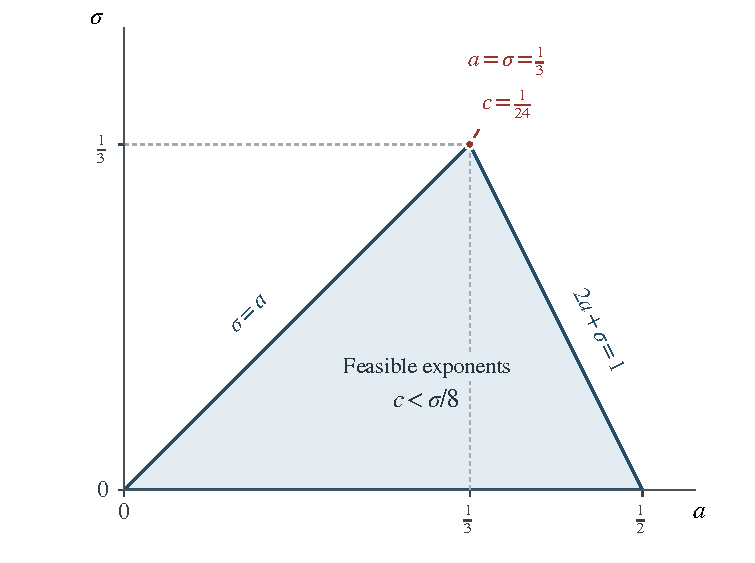
\includegraphics[width=.82\textwidth]{figures/parameter_region.pdf}
 \caption{The closed power-exponent region
 \(0\le\sigma\le a\), \(2a+\sigma\le1\).
 Strict interior choices give the fixed-power construction.
 Logarithmic factors implement the limiting vertex in the endpoint
 theorem. This is the feasible region of the displayed estimates,
 not a lower bound on the complexity of every possible refinement.}
 \label{fig:parameters}
\end{figure}

The logarithmic choices can be understood from the same calculation.
For a small tolerance \(\zeta\), the local-lemma cutoff is of size
\(D\log k/\zeta^2\). The two dominant signature estimates are
of respective sizes
\[
 \frac{D^2\log k}{\zeta^2},
 \qquad \frac{k\log k}{D}.
\]
Equating them suggests \(D\asymp k^{1/3}\zeta^{2/3}\),
and then \(pk\asymp k^{2/3}(\log k)\zeta^{-2/3}\).
Choosing \(\zeta\asymp1/\log k\) keeps the outer-balance loss
of order \(k\) while giving
\[
 \log(1/p)=\tfrac13\log k-\tfrac53\log\log k-O(1).
\]
The binary rich estimate uses approximately
\((k/8)\log(1/p)\) as its size budget, explaining both \(1/24\)
and \(5/24\).
The proofs above establish that these choices work.
They do not establish that either coefficient is an intrinsic
barrier: smaller actual pattern counts, stronger dependence
information, or a different key could change the ledger.
